\section{Baseline I/O Performance} \label{sec:results}

\begin{figure}[t]
    \centering
    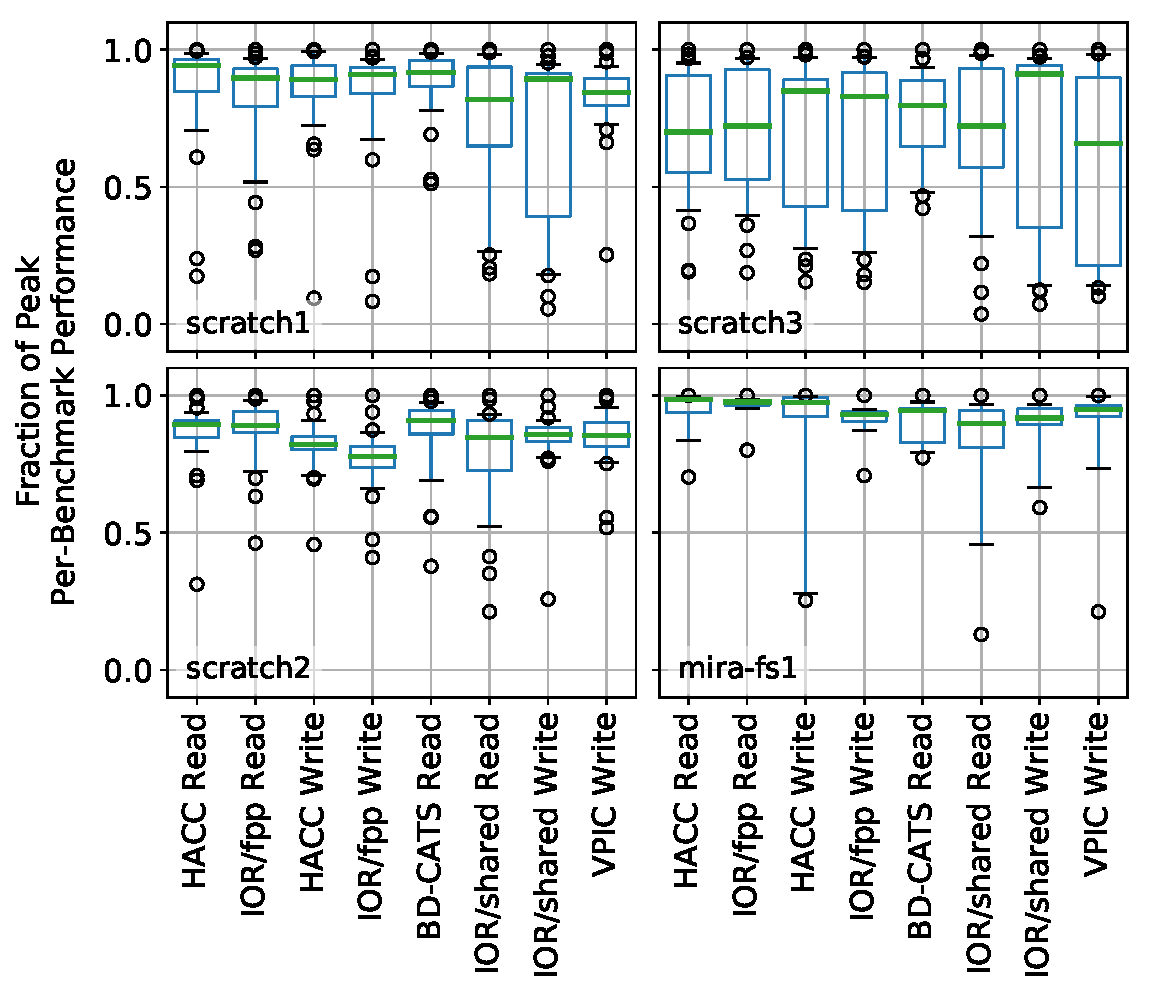
\includegraphics[width=1.0\columnwidth]{figs/perf-boxplots.pdf}
    \vspace{-.25in}
    \caption{I/O performance grouped by test applications and read(R)/write(W) mode.  Whiskers represent the 5th and 95th percentiles.}
    \label{fig:perf-summary-boxplots-motif}
    \vspace{-.3in}
\end{figure}

Because variation in peak I/O performance is caused by different I/O access patterns~\cite{Lofstead2010,Uselton2010,Xie2012}, we first establish the baseline variation of each benchmark on each system.
We define the \emph{fraction of peak performance} as the observed I/O bandwidth (performance) of a job divided by the maximum performance observed for all jobs \emph{of the same I/O motif} as listed in Table \ref{tab:bench-config} and whether the job read or wrote.
% For example, the fraction peak performance for a HACC write test is normalized to the highest performance of any HACC write test on the same file system.

The distribution of fraction peak performance (Figure~\ref{fig:perf-summary-boxplots-motif})
reveals that the degree of variation \emph{within} each application varies with each file system.
For example, the HACC write workload is susceptible to a long tail of performance loss on mira-fs1 despite mira-fs1's overall lower variation as evidenced by the distance between all I/O motifs' whiskers relative to the Edison file systems.
Edison's scratch3 also demonstrates broad performance variation for the VPIC write workload, contrasting with the narrower variation of this application on other systems.  We conclude that such variability is the result of factors intrinsic to both the application and the file system;
different I/O motifs result in different levels of performance \emph{and} variability.

Furthermore, Figure~\ref{fig:perf-summary-boxplots-motif} shows that variation is not only a function of the file system architecture; all Edison file systems are Lustre-based, yet Figure~\ref{fig:perf-summary-boxplots-motif} shows a marked difference in variability between scratch1/scratch2 and scratch3.
Thus, these differences in performance variation must be a function of differences in three factors of the I/O subsystem:
(1) hardware architecture, evident when comparing the distributions of mira-fs1 performance to Edison;
(2) application I/O patterns, evident from the variation within any single file system; and
(3) overall file system climate, evident by comparing the architecturally equivalent Edison scratch1/scratch2 with scratch3 file systems.
% \begin{enumerate}[leftmargin=*]
% \item Hardware architecture, evident when comparing the distributions of mira-fs1 performance to Edison
% \item Application I/O patterns, evident from the variation within any single file system
% \item Overall file system climate, evident by comparing the architecturally equivalent Edison scratch1/scratch2 with scratch3 file systems
% \end{enumerate}

This finding underscores the importance of examining multiple sources of I/O characterization data (e.g., application-level and server-side) in concert and with historical context in order to develop a full understanding of I/O performance.

%%%%%%%%%%%%%%%%%%%%%%%%%%%%%%%%%%%%%%%%%%%%%%%%%%%%%%%%%%%%%%%%%%%%%%%%%%%%%%%%
\section{Integrated Analysis} \label{sec:results/umami}
%%%%%%%%%%%%%%%%%%%%%%%%%%%%%%%%%%%%%%%%%%%%%%%%%%%%%%%%%%%%%%%%%%%%%%%%%%%%%%%%

With an understanding of the baseline performance variation on each system and application, we then consider metrics from the sources described in Section \ref{sec:methods} to analyze how extrinsic factors affect performance.
Bandwidth contention from other jobs is an intuitive source of performance variation, so we define the \emph{bandwidth coverage factor} ($\mathit{CF}_{\mathit{bw}}$) of a job $j$ to quantify the effects of competing I/O traffic:

\begin{equation} \label{eq:cf}
    \mathit{CF}_{\mathit{bw}}(j) = \frac{N_{\textup{bytes}}^{\textup{Darshan}}(j)}
    {\sum_{t,s}^{\textup{time,servers}}
    \left [ N_{\textup{bytes}}^{\textup{LMT,ggiostat}}(t,s) \right ] , }
\end{equation}
%
where 
$N_{\textup{bytes}}^{\textup{Darshan}}$ are the bytes read and written by job $j$ according to its Darshan log and 
$N_{\textup{bytes}}^{\textup{LMT,ggiostat}}$ are the bytes read and written to a parallel file system server $s$ during a 5-second time interval $t$.
The time interval over which the job ran ($\mathit{time}$) and the servers to which the job wrote ($\mathit{servers}$) are also stored in the job's Darshan log~\cite{snyder2016modular}.
$\mathit{CF}_{\mathit{bw}}$ is a direct reflection of how much I/O traffic a job competed against in the underlying file systems.
When $\mathit{CF}_{\mathit{bw}} = 1.0$, all the server-side I/O can be attributed to job $j$, whereas $\mathit{CF}_{\mathit{bw}} = 0.5$ indicates that only half of the server-side I/O is attributable to job $j$ while the other half is from other sources.

$\mathit{CF}_{\mathit{bw}}$ can be generalized to any metric for which the contribution of an individual job can be distinguished from the system-level aggregate.
As such, we also define $\mathit{CF}_{\mathit{IOPS}}$ of IOPS (derived from Darshan and ggiostat) and $\mathit{CF}_{\mathit{nodehrs}}$ of node-hours (derived from job-scheduling data).

%In practice, $\mathit{CF}$ can be slightly greater than $1.0$ as a result of two conditions:
%a) when the storage system traffic monitoring (LMT/ggiostat) does not capture data from all servers during a polling interval, or
%b) when clock skew between the compute nodes and the file system servers causes the Darshan log and LMT/ggiostat to have an inconsistent understanding of when I/O happened.
%In this study, such noise never resulted in $\mathit{CF} > 1.2$.
%%%% GKL: The ratio of CF > 1.2 to all CF measurements is very high on Mira; 96 of the 214 measurements provided by Shane were dropped due to this filter criterion

$\mathit{CF}$, system health data, and job topology data let us contextualize performance anomalies and quantify where a job's I/O performance falls on the spectrum of normalcy relative to jobs with similar motifs.
To concisely display this information and identify metrics that most likely contribute to abnormal performance, we propose a unified monitoring and metrics interface (UMAMI) diagram as demonstrated in Figure \ref{fig:umami-scratch2-hacc-write}.
UMAMI presents historic measurements (the I/O climate) alongside a box plot that summarizes each metric.
% \todo{ROB: It would be easy enough to generalize to any point in the time series, rather than terminating at the job of interest, allowing one to show how the weather at some prior point in time fits into the climate beyond the job, too (i.e., just put the star wherever it belongs in the timeline?).}
These time series plots highlight a job of interest and define the I/O weather at the time that job ran.

Overlaying this weather on the climate (dashed lines in the box plots) shows how each metric compares with the distribution of weather conditions before, after, or surrounding the job of interest to enable rapid differentiation of rare events from long-term performance problems.
In the remainder of this section we use UMAMI diagrams to identify different factors that do and do not contribute to I/O performance loss.
{Although we collected 58 metrics for each job, we chose only the most relevant metrics to include in each UMAMI diagram based on (1) which metrics most strongly correlated with performance, and (2) which metrics we expected to affect performance but did not.

These case studies were performed on Mira and Edison, but UMAMI's modularity allow it to analyze a variety of data sources and enables portable deployment for production use.

\begin{figure}[t]
    \centering
    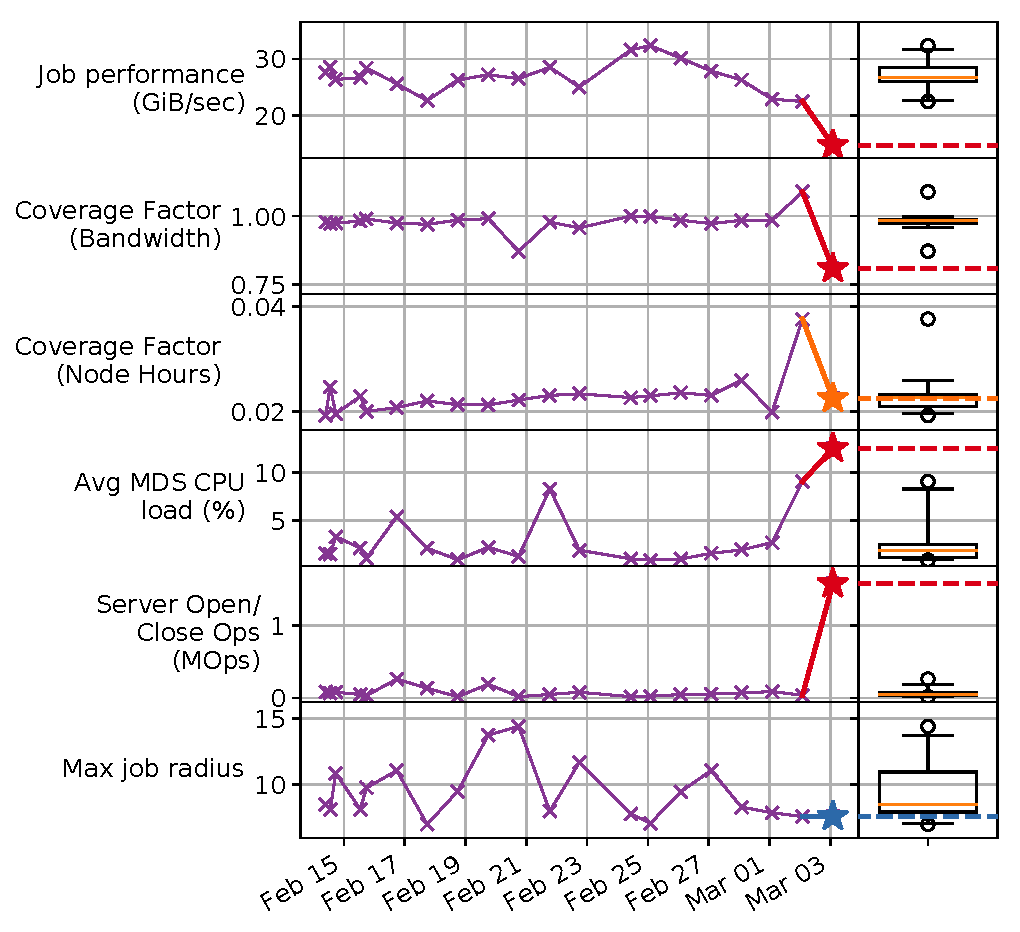
\includegraphics[width=1.0\columnwidth]{figs/umami-scratch2-hacc-write.pdf}
    \vspace{-.25in}
    \caption{UMAMI of HACC write workloads on Edison scratch2.
    Left panes show measurements from previous runs of the same motif and are summarized to the right.
    Stars highlight the job of interest and are colored according to the quartile in which they fall (red being the worst and blue the best).
    Whiskers indicate 5th and 95th percentiles; circles are outliers.}
    \label{fig:umami-scratch2-hacc-write}
    \vspace{-.2in}
\end{figure}

%%%%%%%%%%%%%%%%%%%%%%%%%%%%%%%%%%%%%%%%%%%%%%%%%%%%%%%%%%%%%%%%%%%%%%%%%%%%%%%%
\subsection{Case study: I/O contention}
%%%%%%%%%%%%%%%%%%%%%%%%%%%%%%%%%%%%%%%%%%%%%%%%%%%%%%%%%%%%%%%%%%%%%%%%%%%%%%%%

The UMAMI example in Figure \ref{fig:umami-scratch2-hacc-write} represents a HACC write test whose job performance measurement relative to previous HACC write jobs indicate statistically abnormal performance.
This poor performance was accompanied by an unusually low $\mathit{CF}_{\mathit{bw}}$ and high metadata load, highlighted as red dashed lines in the box plots that denote their place in the least-favorable quartile of past measurements.

Conversely, the maximum job radius fell into the most favorable quartile (indicated by the blue dashed line),
and the number of concurrently running jobs ($\mathit{CF}_{\mathit{nodehrs}}$) was not abnormally large.
Because normal performance was often observed even in cases when both of these metrics were abnormally poor, we conclude that the maximum job radius and $\mathit{CF}_{\mathit{nodehrs}}$ metrics are too coarse-grained to indicate poor performance, and
more insight into what resources the competing jobs were actually consuming when each HACC job ran are required.
Given this body of information, we attribute this HACC job's poor performance to I/O loads from other jobs that competed for both bandwidth and metadata rates.

%%%%%%%%%%%%%%%%%%%%%%%%%%%%%%%%%%%%%%%%%%%%%%%%%%%%%%%%%%%%%%%%%%%%%%%%%%%%%%%%
\subsection{Case study: metadata load}
%%%%%%%%%%%%%%%%%%%%%%%%%%%%%%%%%%%%%%%%%%%%%%%%%%%%%%%%%%%%%%%%%%%%%%%%%%%%%%%%

\begin{figure}[t]
    \centering
    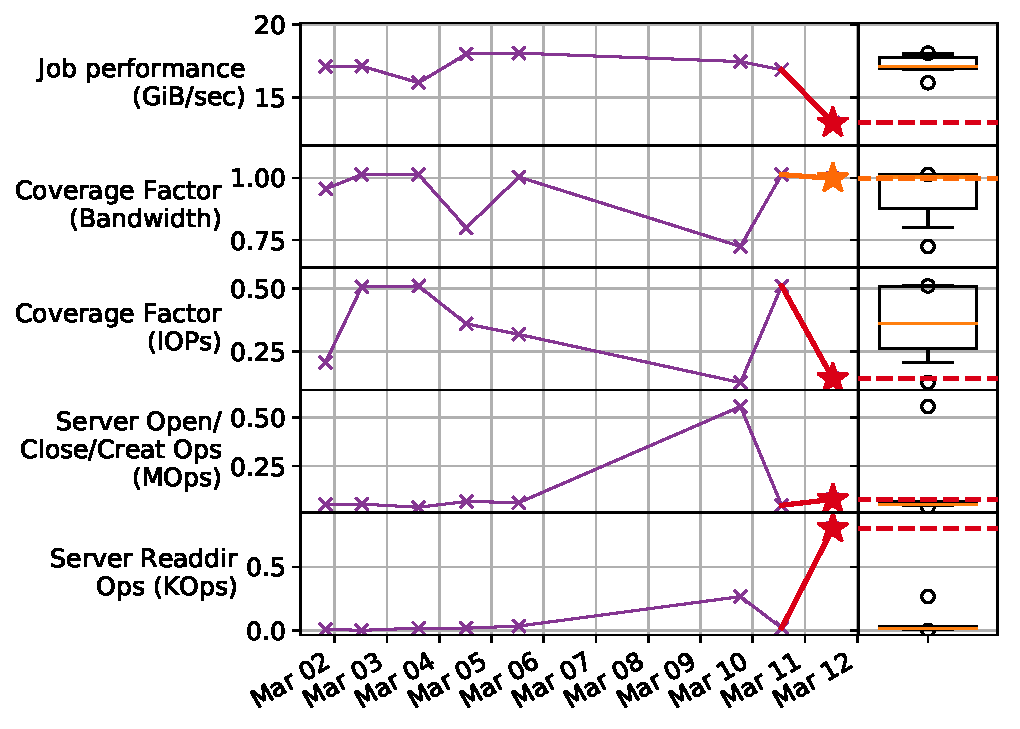
\includegraphics[width=1.0\columnwidth]{figs/umami-mira-fs1-vpic-write.pdf}
    \vspace{-.25in}
    \caption{UMAMI demonstrating the climate surrounding VPIC write workloads on Mira compared with a most recent run, which showed highly unusual weather in the form of an excess of \texttt{readdir(3)} calls.
    }
    \label{fig:umami-mira-fs1-vpic-write}
    \vspace{-.15in}
\end{figure}

Figure \ref{fig:umami-mira-fs1-vpic-write} shows the UMAMI diagram for a poorly performing VPIC workload.
$\mathit{CF}_{\mathit{bw}}$ is within normal parameters, indicating normal (minimal) levels of bandwidth contention.
$\mathit{CF}_{\mathit{IOPS}}$ is abnormally low, although previous values have been equally low despite a lack of dramatic performance loss (e.g., on March 1 and March 9).
The only metric that shows a unique, undesirable value is the number of readdir operations handled by the file system, indicating a file system traversal was running concurrently with this VPIC job.
From this we infer that metadata load, not bandwidth contention, contributed to poor VPIC performance on March 11.

%%%%%%%%%%%%%%%%%%%%%%%%%%%%%%%%%%%%%%%%%%%%%%%%%%%%%%%%%%%%%%%%%%%%%%%%%%%%%%%%
\subsection{Case study: storage capacity}
%%%%%%%%%%%%%%%%%%%%%%%%%%%%%%%%%%%%%%%%%%%%%%%%%%%%%%%%%%%%%%%%%%%%%%%%%%%%%%%%

\begin{figure}[t]
    \centering
    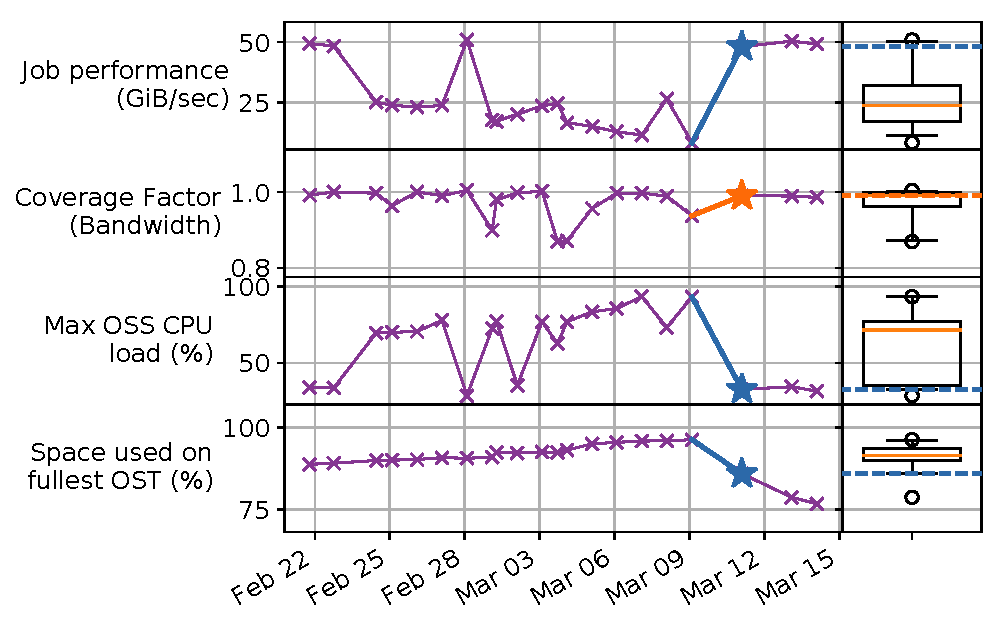
\includegraphics[width=1.0\columnwidth]{figs/umami-scratch3-hacc-write-long-term.pdf}
    \vspace{-.25in}
    \caption{UMAMI of HACC write performance on Edison's scratch3 file system showing a longer-term period of performance degradation that was associated with poor file system health.
%   Significance of each pane and its contents are the same as explained in Figure \ref{fig:umami-scratch2-hacc-write}.
    }
    \label{fig:umami-scratch3-hacc-write-long-term}
	\vspace{-.15in}
\end{figure}

This holistic approach can also identify long-term performance degradation.
Figure \ref{fig:umami-scratch3-hacc-write-long-term} shows the UMAMI of HACC on Edison scratch3 when $CF$s were not unusual despite an ongoing $2\times$ slowdown over the normal 50 GiB/sec between February 24 and March 9.
The magnitude of performance loss closely followed the maximum CPU load on the Lustre OSSes, and this period also coincided with  scratch3 OSTs approaching 100\% fullness.
The relationship between CPU load, OST fullness, and I/O performance points to an increasing cost of scavenging empty blocks on writes, and this behavior is consistent with known performance losses that result from Lustre OSTs filling~\cite{oral2014best}.
Furthermore, I/O performance was restored on March 9 which is when NERSC staff initiated a file system purge.
Thus, we conclude that this long-term performance degradation was the result of poor file system health resulting from Edison scratch3 being critically full.
